\chapter{Formulating a Mathematical Model}
based on DAE lecture and modelling and discretiztation of elec circuit problems.

To accurately represent a physical system in a mathematical model we first have to think about \textbf{how} to best formulate a mathematical model that foormulates this system.
This chapter aims to elaborate on the Modified Nodal Analysis (MNA) of an electrical circuit. For this we have to introduce the notions of network topology as well as some basic electrical components and laws.

\section{Network Topology}
An electrical circuit is usually considered as a graph $(N,E)$ where $N = (n_0, n_1, n_2, ...)$ are the Nodes and $E = (e_{ij})_{ij}$ are the edges.For some $i$ and some $j$ we have that $e_{ij} = (n_j, n_k)$ is the edge from node $j$ to node $k$.
We can store this information in an \emph{incidence matrix} $\tilde{A} = (\tilde{a}_{ij})_{ij}$ which is defined by
\begin{displaymath}
	\tilde{a}_{ij} = 
	\begin{cases}
		1 &   \text{edge $j$ starts at node $i$},\\
		-1 &  \text{edge $j$  ends at node $i$},\\
		0 & \text{else}.				
	\end{cases}
\end{displaymath}
We call $u = (u_0, u_1, u_2, ...)$ the corresponding potentials to the nodes $N$. The difference between the potentials at two connected nodes is called the voltage at the respective edge. To fix the absolute values of these potentials we have to set one node to a fixed potential. We will do that by ``grounding'' the node $n_0$, this means we set the potential $u_0 := 0$. This grounding of a node allows us to remove the corresponding row from the incidence matrix to get the \emph{reduced incidence matrix} $A$. The vector $v = (v_{ij})_{ij}$ represents the voltages at the edges. For some $i$ and some $j$ the voltage at edge $ij$ is $v_{ij} = u_i - u_j$.

We will later see, that the components of an electrical crircuit, which will be installed along the edges, describe a relationship between the edges current and its voltage. Thus a current vector $i = (i_1, i_2, i_3, ...)$ containing the currents along the edges is required.

\textbf{example}

\section{Energy Conservation Laws}
To fully fix all the variables that arrise in the model of an electrical circuit we will need some \emph{conservation laws}:
\begin{itemize}
	\item \textbf{Kirchhoff's voltage law (KVL):} \newline
	The sum of voltages along each loop of the network must equal to zero. Using the incidence matrix $A$ this law can be formulated as
	\begin{equation}
		\label{KVL}
		A^\top * u = v.
	\end{equation}
	\item \textbf{Kirchhoff's current law (KCL):} \newline
	For any node, the sum of currents flowing into the node is equal to the sum of currents flowing out of the node. Using the incidence matrix $A$ again, this law can be formulated as
	\begin{equation}
		\label{KCL}
		A * i = 0.
	\end{equation}
\end{itemize}

\section{Electrical Components and their relations}
Electrical components are described by equations relating their edge voltage $v$ to their edge current $i$. We will mainly focus on so called RLC-networks which consist of resistors, capacitors, inductances, voltage sources and current sources. Diodes and Transistors as well as other electrical components can be described in a similar way, although these would lead to a more difficult analysis of the system.
\begin{itemize}
	\item \textbf{Resistor} \newline
	Resistors ''resist`` the flow of current, which causes voltage to drop. This behaviour is described by the \emph{resistance} $R$ which is given in \emph{Ohm} ($\Omega$) and its reciprocal, the \emph{conductance} $G$, which is given in \emph{Simens} ($S=\frac{1}{\Omega}$). 
	\begin{displaymath}
		v = R*i \quad \text{or} \quad i = G*u.
	\end{displaymath}
	\begin{figure}[H]
		\label{fig:resistor symbol}
		\centering
		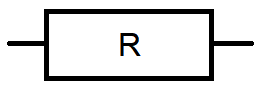
\includegraphics[width=2cm]{pictures/resistor.png}
		\caption{resistor symbol}
	\end{figure}
	\item \textbf{Capacitor} \newline
	Capacitors ''store`` electrical energy by accumulating electrical charge. Their characteristic equations can be described directly using the stored charge $Q$ or indirectly using the change in charge, which is nothing other than the current $I$. The \emph{capacitance} $C$ is given in \emph{Farads} ($F$).
	\begin{displaymath}
		Q = C * v \quad \text{and by derivation in t} \quad I = C*\dot{v}.
	\end{displaymath}
	\begin{figure}[H]
		\label{fig:capacitor symbol}
		\centering
		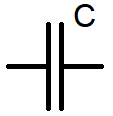
\includegraphics[width=2cm]{pictures/capacitor.png}
		\caption{capacitor symbol}
	\end{figure}
	\item \textbf{Inductor (Coil)} \newline
	An electric current flowing through a conductor generates a magnetic field $\Phi$ surrounding it. This magnetic field causes a voltage drop dependant on the change in current. The \emph{inductance} $L$ is given in \emph{Henry} ($H$).
	\begin{displaymath}
		\Phi = L*i \quad \text{and by derivation in t} \quad v = L*\dot{i}.
	\end{displaymath}
	\begin{figure}[H]
		\label{fig:inductor symbol}
		\centering
		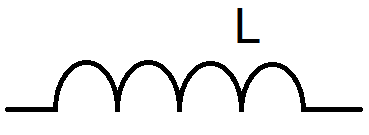
\includegraphics[width=3cm]{pictures/inductance.png}
		\caption{inductor symbol}
	\end{figure}
	\item \textbf{Voltage Source} \newline
	A voltage source supplies the system with a voltage. It can either supply varying amounts of voltage (with the special case of alternating current AC) or a fixed amount of voltage. The unit of voltage is \emph{Volts} ($V$).
	\begin{displaymath}
		v = v_{src}
	\end{displaymath}
	\begin{figure}[H]
		\label{fig:voltage source symbol}
		\centering
		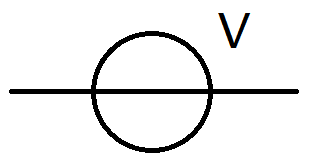
\includegraphics[width=4cm]{pictures/voltage_source.png}
		\caption{voltage source symbol}
	\end{figure}
	\item \textbf{Current Source} \newline
	A current source supplies the system with current. It can either supply varying amounts of current (with the special case of alternating current AC) or a fixed amount of current. The unit of current is \emph{Ampere} ($A$).
	\begin{displaymath}
		i = i_{src}
	\end{displaymath}
	\begin{figure}[H]
		\label{fig:current source symbol}
		\centering
		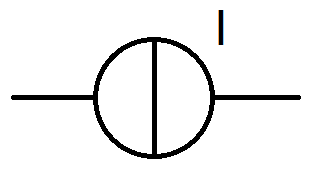
\includegraphics[width=4cm]{pictures/current_source.png}
		\caption{current source symbol}
	\end{figure}
	\item Diode - to be filled with information after the rest is complete
	\item Transistor - unlike the other components which where all two-teminal components a transisstor is a three-terminal component
\end{itemize}

\section{Modified Nodal Analysis - MNA}

num gew dgl steif n steif - seite 422 \newline
modelling discr circ prob - seite 19

To analyse the network further we will sort the reduced incidence matrix $A$ such that is has the block form
\begin{displaymath}
	A = (A_R A_C A_L A_V A_I)
\end{displaymath}
where $A_R$, $A_C$, $A_L$, $A_V$ and $A_I$ all include the collumns that are related to the resistors, capacitors, coils, voltage sources and current sources. 

To mathematically describe the circuit we will use \emph{modified nodal analysis} (or short MNA). MNA uses the node voltages as well as the currents of the coils and the voltage sources as unknowns and is based on the conservation laws \ref{KCL} and \ref{KVL} as well as on the voltage-current relations of the electrical components. By replacing all edge-currents with their respective voltage-current relation and ell egde-voltages with their node-potentials we obtain the MNA-equations

\begin{displaymath}
	\begin{aligned}
		A_C C A_C^\top \dot{u} + A_R G A_R^\top u + A_L i_L + A_V i_V + A_I i_{src} &= 0 , \\
		L \dot{i_L}	- A_L^\top u &= 0 , \\
		-A_V^\top + v_{src} &= 0.
	\end{aligned}	
\end{displaymath}
In matrix form these read as
\begin{equation}
	\label{MNA_Matrixform}
	\begin{pmatrix}
		A_C C A_C^\top & 0 & 0 \\
		0 & L & 0 \\
		0 & 0 & 0
	\end{pmatrix}
	*
	\begin{pmatrix}
		\dot{u} \\
		\dot{i_L} \\
		\dot{i_V}
	\end{pmatrix}
	+
	\begin{pmatrix}
		A_R G A_R^\top & A_L & A_V \\
		-A_L^\top & 0 & 0 \\
		-A_V^\top & 0 & 0 
	\end{pmatrix}
	*
	\begin{pmatrix}
		u \\
		i_L \\
		i_V
	\end{pmatrix}
	=
	\begin{pmatrix}
		-A_I i_{src} \\
		0 \\
		-v_{src}
	\end{pmatrix} , 
\end{equation}
where the diagonal matrices $C$, $G$ and $L$ contain the capacities, conductivities and inductivities.

The resulting systems are \emph{stiff} systems. This means that for their numerical solution special care has to be put into which methods are suitable for a solving these sytsems in a stable manner.

\textbf{example}

\section{Charge/Flux oriented formulation of MNA}
may noot be too importatn - leave out?

Again using KCL \ref{KCL} and the component equations we formulate a system of equations. (\textbf{more here}) What is flux and charge - explain either here or witht the components

\begin{align}
	A_C\dot{q} + A_R r(A_R^\top u,t) + A_L i_L + A_V i_V + A_I i(A^\top u, \dot{q}, i_L, i_V, t) &= 0 \label{charge/flux-1} \\
	\dot{\phi} - A_L^\top u &= 0 \label{charge/flux-2} \\
	v(A^\top u, \dot{q}, i_L, i_V, t) - A_V^\top u &= 0 \label{charge/flux-3} \\
	q - q_C(A_C^\top u) &= 0 \label{charge/flux-4} \\
	\phi - \phi_L(i_L) &= 0  \label{charge/flux-5} 
\end{align}

Using
\begin{description}
	\item node potentials $u$,
	\item branch currents through voltage and flux controlled elements $i_V$ and $i_L$,
	\item charges and fluxes $q$ and $\phi$,
	\item voltage dependent resistors $r$,
	\item voltage and current dependent charge and flux sources $q_C$ and $\phi_L$,
	\item controlled current and voltage sources $i_{src}$ and $v_{src}$.
\end{description} 

\begin{figure}[H]
	\centering
	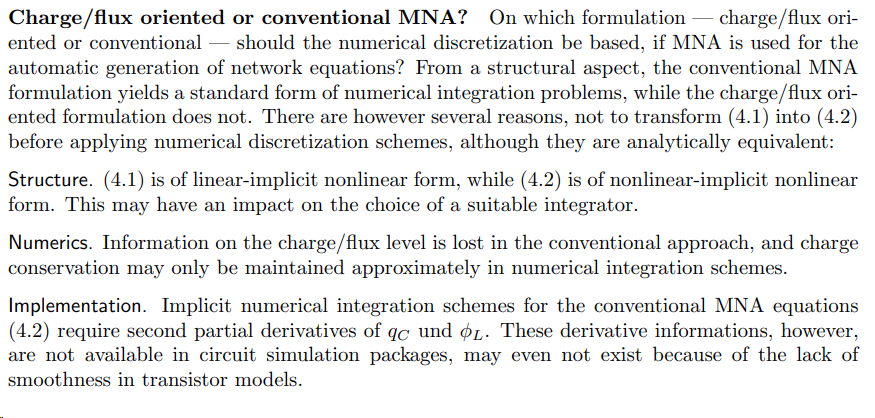
\includegraphics[width=0.7\linewidth]{screenshot007}
	\caption{}
	\label{fig:screenshot007}
\end{figure}

so it makes sense to use the conventional approach of MNA - compare with phd thesis 